\documentclass[class=minimal,border=0pt]{standalone}
\usepackage{tikz}
\usetikzlibrary{arrows.meta}
\begin{document}
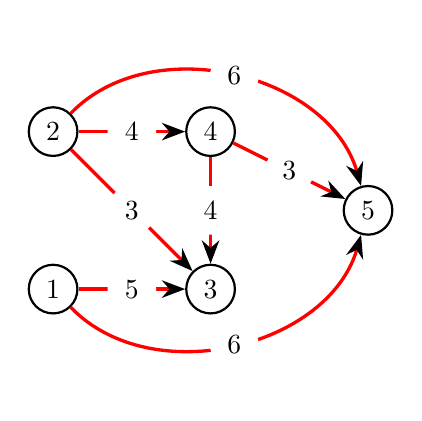
\begin{tikzpicture}
\begin{scope}[every node/.style={circle,thick,draw}]
    \node (1) at (0,0) {1};
    \node (2) at (0,2) {2};
    \node (3) at (2,0) {3};
    \node (4) at (2,2) {4};
    \node (5) at (4,1) {5};
\end{scope}

\begin{scope}[>={Stealth[black]},
              every node/.style={fill=white,circle},
              every edge/.style={draw=red,very thick}]
    \path [->] (1) edge node {$5$} (3);
    \path [->] (2) edge node {$3$} (3);
    \path [->] (2) edge node {$4$} (4);
    \path [->] (4) edge node {$4$} (3);
    \path [->] (4) edge node {$3$} (5);
    \path [->] (1) edge[bend right=60] node {$6$} (5);
    \path [->] (2) edge[bend left =60] node {$6$} (5);
\end{scope}
\end{tikzpicture}
\end{document}
